\documentclass[a4paper, 12pt]{report}		% general format
\usepackage{multicol}
%%%% Charset
\usepackage{cmap}							% make PDF files searchable and copyable
\usepackage{bm}
\usepackage{pdfpages}
\usepackage[utf8x]{inputenc} 				% accept different input encodings
\usepackage[english,russian]{babel}   %% загружает пакет многоязыковой вёрстки
%\usepackage{fontspec}      %% подготавливает загрузку шрифтов Open Type, True Type и др.
%\defaultfontfeatures{Ligatures={TeX},Renderer=Basic}  %% свойства шрифтов по умолчанию
%\setmainfont[Ligatures={TeX,Historic}]{Roboto-Light} %% задаёт основной шрифт документа
%\setsansfont{Roboto-Light}  
\usepackage{float}
%%%% Graphics
%\usepackage[dvipsnames]{xcolor}			% driver-independent color extensions
\usepackage{graphicx}						% enhanced support for graphics
\usepackage{wrapfig}						% produces figures which text can flow around

%%%% Math
\usepackage{amsmath}						% American Mathematical Society (AMS) math facilities
\usepackage{amsfonts}						% fonts from the AMS
\usepackage{amssymb}						% additional math symbols

%%%% Typograpy (don't forget about cm-super)
\usepackage{microtype}						% subliminal refinements towards typographical perfection
\linespread{1.0}							% line spacing
\usepackage[mag=1000, left=2.0cm, right=1.5cm, top=2cm, bottom=2cm, headsep=0.7cm, footskip=1cm]{geometry}
\setlength{\parindent}{0pt}					% we don't want any paragraph indentation
\usepackage{parskip}						% some distance between paragraphs

%%%% Tables
\usepackage{tabularx}						% tables with variable width columns
\usepackage{multirow}						% for tabularx
\usepackage{hhline}							% for tabularx
\usepackage{tabu}
\usepackage{longtable}

%%%% Graph
\usepackage{tikz}							% package for creating graphics programmatically
\usetikzlibrary{arrows}						% edges for tikz

%%%% Other
\usepackage{url}							% verbatim with URL-sensitive line breaks
\usepackage{fancyvrb}						% sophisticated verbatim text (with box)

\usepackage{fancyhdr}
\usepackage{latexsym}
\usepackage{booktabs}
\usepackage{array}

\usepackage{listings}
\usepackage{caption}
\DeclareCaptionFont{white}{\color{white}}
\DeclareCaptionFormat{listing}{\colorbox{gray}{\parbox{\dimexpr\textwidth-1.72\fboxsep\relax}{#1#2#3}}}
\captionsetup[lstlisting]{format=listing,labelfont=white,textfont=white,margin=0pt}
\lstset{language=C,
	basicstyle=\footnotesize,
	keepspaces=true,
	tabsize=4,               
	frame=single,                           % Single frame around code
	rulecolor=\color{black},
	captionpos=b,
	showstringspaces=false,	
	abovecaptionskip=-0.9pt,
	xleftmargin=3.4pt,
	xrightmargin=2.6pt,
	breaklines=true,
	postbreak=\raisebox{0ex}[0ex][0ex]{\ensuremath{\color{black}\hookrightarrow\space}},
	xleftmargin=3.2pt,
	literate={а}{{\selectfont\char224}}1
	{~}{{\textasciitilde}}1
	{б}{{\selectfont\char225}}1
	{в}{{\selectfont\char226}}1
	{г}{{\selectfont\char227}}1
	{д}{{\selectfont\char228}}1
	{е}{{\selectfont\char229}}1
	{ё}{{\"e}}1
	{ж}{{\selectfont\char230}}1
	{з}{{\selectfont\char231}}1
	{и}{{\selectfont\char232}}1
	{й}{{\selectfont\char233}}1
	{к}{{\selectfont\char234}}1
	{л}{{\selectfont\char235}}1
	{м}{{\selectfont\char236}}1
	{н}{{\selectfont\char237}}1
	{о}{{\selectfont\char238}}1
	{п}{{\selectfont\char239}}1
	{р}{{\selectfont\char240}}1
	{с}{{\selectfont\char241}}1
	{т}{{\selectfont\char242}}1
	{у}{{\selectfont\char243}}1
	{ф}{{\selectfont\char244}}1
	{х}{{\selectfont\char245}}1
	{ц}{{\selectfont\char246}}1
	{ч}{{\selectfont\char247}}1
	{ш}{{\selectfont\char248}}1
	{щ}{{\selectfont\char249}}1
	{ъ}{{\selectfont\char250}}1
	{ы}{{\selectfont\char251}}1
	{ь}{{\selectfont\char252}}1
	{э}{{\selectfont\char253}}1
	{ю}{{\selectfont\char254}}1
	{я}{{\selectfont\char255}}1
	{А}{{\selectfont\char192}}1
	{Б}{{\selectfont\char193}}1
	{В}{{\selectfont\char194}}1
	{Г}{{\selectfont\char195}}1
	{Д}{{\selectfont\char196}}1
	{Е}{{\selectfont\char197}}1
	{Ё}{{\"E}}1
	{Ж}{{\selectfont\char198}}1
	{З}{{\selectfont\char199}}1
	{И}{{\selectfont\char200}}1
	{Й}{{\selectfont\char201}}1
	{К}{{\selectfont\char202}}1
	{Л}{{\selectfont\char203}}1
	{М}{{\selectfont\char204}}1
	{Н}{{\selectfont\char205}}1
	{О}{{\selectfont\char206}}1
	{П}{{\selectfont\char207}}1
	{Р}{{\selectfont\char208}}1
	{С}{{\selectfont\char209}}1
	{Т}{{\selectfont\char210}}1
	{У}{{\selectfont\char211}}1
	{Ф}{{\selectfont\char212}}1
	{Х}{{\selectfont\char213}}1
	{Ц}{{\selectfont\char214}}1
	{Ч}{{\selectfont\char215}}1
	{Ш}{{\selectfont\char216}}1
	{Щ}{{\selectfont\char217}}1
	{Ъ}{{\selectfont\char218}}1
	{Ы}{{\selectfont\char219}}1
	{Ь}{{\selectfont\char220}}1
	{Э}{{\selectfont\char221}}1
	{Ю}{{\selectfont\char222}}1
	{Я}{{\selectfont\char223}}1,
	extendedchars=true
}

%галочка
\usepackage{amssymb}% http://ctan.org/pkg/amssymb
\usepackage{pifont}% http://ctan.org/pkg/pifont
\newcommand{\cmark}{\ding{52}}%
\newcommand{\xmark}{\ding{56}}
%------------------------------------------------------------------------------
\renewcommand{\labelenumii}{\theenumii}
\renewcommand{\theenumii}{\theenumi.\arabic{enumii}.}
\addto\captionsrussian{\def\refname{Список использованных источников}}
\begin{document}
\begin{titlepage}
\thispagestyle{empty}

\begin{center}
Санкт-Петербургский политехнический университет Петра Великого\\
Институт Информационных Технологий и Управления\\*
Кафедра компьютерных систем и программных технологий\\*
\hrulefill
\end{center}

\vspace{15em}

\begin{center}
\textsc{\textbf{Курсовая работа}}
\vspace{1em}

Дисциплина: \textbf{Методы оптимизации}
\vspace{2em}

Тема: \textbf{Формулировка и решение задачи выбора оптимального решения с использованием различных математических моделей}
\end{center}

\vspace{16em}

\begin{flushleft}
Выполнил студент гр. 53501/3 \hrulefill С.А. Мартынов \\
\vspace{1.5em}
Руководитель, к.т.н.,доц. \hrulefill А.Г. Сиднев\\
\end{flushleft}

\vspace{\fill}

\begin{center}
Санкт-Петербург \\
2015
\end{center}

\end{titlepage}
\setcounter{page}{2}
\tableofcontents
\clearpage

%------------------------------------------------------------------------------
%\input{intro}
\setcounter{chapter}{2}
\chapter{Поиск оптимальных параметров сети систем массового обслуживания}
\section{Постановка задачи}
\textbf{Вариант:} задача 4, вариант 144.

\tabulinesep = 1mm
\begin{longtabu} to \textwidth {|X[c , m ] |X[4,c , m ] | X[c , m ]|X[c , m ]|X[c , m ]| X[c , m ]|X[4,c , m ]|}\firsthline\hline

№ вар&$Q=\{q_{ij}\}_{\begin{matrix}i=\overline{0,n}\\j=\overline{0,n}\end{matrix}}$&$ca_0$&$\lambda_0$&$L_r$&$\mu$&$\{cs_j\}$\\ \hline
144&$\begin{array}{c|c|c|c|c}0& 0.2& 0.3& 0.2& 0.3\\ \hline 0.1&0&0.2&0.6&0.1\\ \hline 0.6&0.2&0&0.1&0.1\\ \hline 0&0.5&0.1&0&0.4\\ \hline 0.5&0.3&0.1&0.1&0 \end{array}$&0.16&8&-&10&$\begin{array}{c|c|c|c}0.04& 0.04& 0.04& 0.04	\end{array}$\\ \hline
\end{longtabu}

Найти:
\begin{equation*}
min L(\mu)=\sum_{j=1}^{n}L_j
\end{equation*}
При условии:
\begin{equation*}
\sum_{j=1}^{n}\mu_j=\mu
\end{equation*}

\section{Решение}
Вычислим мощность $\mu > \mu_j^1, cs$ и $ca$ для каждой станции.

Скорость прихода задач в узел j: $\lambda_j=\lambda_{0j}+\sum_{i=0}^nq_{ij}\lambda_i, j=0, ..., n$
\begin{equation*}
Q =
 \begin{pmatrix}
  0& 0.2& 0.3& 0.2& 0.3 \\
  0.1&0&0.2&0.6&0.1 \\
  0.6&0.2&0&0.1&0.1  \\
  0&0.5&0.1&0&0.4 \\
  0.5&0.3&0.1&0.1&0
 \end{pmatrix}
\end{equation*}
$\lambda_0=8$\\
$\lambda_1=0.2\lambda_0+0\lambda_1+0.2\lambda_2+0.5\lambda_3+0.3\lambda_4$\\
$\lambda_2=0.3\lambda_0+0.2\lambda_1+0\lambda_2+0.1\lambda_3+0.1\lambda_4$\\
$\lambda_3=0.2\lambda_0+0.6\lambda_1+0.1\lambda_2+0\lambda_3+0.1\lambda_4$\\
$\lambda_4=0.3\lambda_0+0.1\lambda_1+0.1\lambda_2+0.4\lambda_3+0\lambda_4$
\begin{lstlisting}[language={matlab}, caption={Код Matlab}, basicstyle=\ttfamily]
A = [1 0 0 0 0;
 0.2 -1 0.2 0.5 0.3;
 0.3 0.2 -1 0.1 0.1;
 0.2 0.6 0.1 -1 0.1;
 0.3 0.1 0.1 0.4 -1];
b=[8; 0; 0; 0; 0];
lambdaj=A\b
\end{lstlisting}
\begin{lstlisting}[language={matlab}, caption={Результат}, basicstyle=\ttfamily]
lambdaj =
    8.0000
    9.1128
    5.7833
    8.3697
    7.2375
\end{lstlisting}
Проверим полученный результат:
\begin{lstlisting}[language={matlab}, caption={Проверка}, basicstyle=\ttfamily]
>> [ 0 0.1 0.6 0 0.5] * lambdaj

ans =
    8.0000 
\end{lstlisting}
Как и ожидалось, была получена $\lambda_0$.\\Вычислим $ca_j$. Для этого, сперва найдем все $\lambda_{ij}$, где $\lambda_{ij} = \lambda_i*q_{ij}$.
\begin{lstlisting}[language={matlab}, caption={Код Matlab}, basicstyle=\ttfamily]
N=5;
Q = [0 0.2 0.3 0.2 0.3;
 0.1 0 0.2 0.6 0.1;
 0.6 0.2 0 0.1 0.1;
 0 0.5 0.1 0 0.4;
 0.5 0.3 0.1 0.1 0];
lambdaij=[];
for i = 1:N
 for j = 1:N
 lambdaij(i,j) = lambdaj(i)*Q(i, j);
 end
end
 lambdaij
\end{lstlisting}
\begin{lstlisting}[language={matlab}, caption={Результат}, basicstyle=\ttfamily]
lambdaij =

         0    1.6000    2.4000    1.6000    2.4000
    0.9113         0    1.8226    5.4677    0.9113
    3.4700    1.1567         0    0.5783    0.5783
         0    4.1849    0.8370         0    3.3479
    3.6188    2.1713    0.7238    0.7238         0
\end{lstlisting}

\begin{equation*}
\lambda =
 \begin{pmatrix}
  0  &  1.6   & 2.4   & 1.6    &2.4 \\
  0.91&    0   & 1.82  &  5.47  &  0.91 \\
  3.47 &   1.16 &   0   & 0.58   & 0.58  \\
  0    &4.18    &0.84    &0       &3.35 \\
  3.62  &  2.17  &  0.72  &  0.72  &  0
 \end{pmatrix}
\end{equation*}
Решим уравнения по формулам:
\begin{equation*}
ca_j=\frac{\lambda_{0j}}{\lambda_j}ca_{0j}+\sum_{i=1}^{n}\frac{\lambda_{ij}}{\lambda_j}ca_{ij}=\sum_{i=0}^{n}\frac{\lambda_{ij}}{\lambda_j}ca_{ij}
\end{equation*}

\begin{equation*}
cd_{ij}=q_{ij}cd_{ij}+1-q_{ij}
\end{equation*}

\begin{lstlisting}[language={matlab}, caption={Код Matlab}, basicstyle=\ttfamily]
caA = 0;
 caB = [0 0 0 0 0];
for j = 1:N
 for i = 1:N
 caA(j,i) = lambdaij(i,j)/lambdaj(j)*Q(i, j);
 caB(j)=caB(j)+lambdaij(i,j)/lambdaj(j)*(1-Q(i,j));
 end
end
 caA = caA-eye(5);
 caA(1,:) = [1 0 0 0 0];
 caA;
 caA^-1;
 caB = -caB';
 caB(1)=0.49;
 caj = (caA^-1)*caB
\end{lstlisting}
\begin{lstlisting}[language={matlab}, caption={Результат}, basicstyle=\ttfamily]
caj =
    0.1600
    0.9486
    0.8902
    0.9461
    0.9049
\end{lstlisting}
Вычислим $L_j$ и $P_j$
\begin{equation*}
p_j=\frac{\lambda_j}{\mu_jm_j}
\end{equation*}
\begin{equation*}
L_j(\lambda_j, ca_j, \mu_j, cs_j)=\frac{(\frac{\lambda_j}{\mu_j})^2(ca_j+cs_j)*g(\lambda_j, ca_j, \mu_j, cs_j)}{2(1-\frac{\lambda_j}{\mu_j})}+\frac{\lambda_j}{\mu_j}
\end{equation*}
\begin{equation*}
PI_j(\mu_j)=-V_j\frac{\partial L_j(\mu_j)}{\partial(\mu_j)}
\end{equation*}
Где:
\begin{equation*}
\lambda_j=9.1128, ca_0=0.16, cs_1=0.04
\end{equation*}
Для этого был написан скрипт matlab.
\begin{lstlisting}[language={matlab}, caption={Код Matlab}, basicstyle=\ttfamily]
for i = 2:N
 [Lj(i-1), Pj(i-1)] = params(lambdaj(i), caj(i), m(i-1), cs(i-1));
end
 Lj
 Pj
 L = sum(Lj)

function [ fLj, fPj ] = params( fl, fca, fm, fcs )
 Lj = '(l/m)^2*(ca+csj)*exp(-2*(1-l/m)*(1-ca)^2/(3*(l/m)*(ca+csj)))/(2*(1-l/m))';
 syms m;
 syms l;
 syms ca;
 syms csj;
 fLj = subs(Lj,l, fl);
 fLj = subs(fLj,m, fm);
 fLj = subs(fLj,ca, fca);
 fLj = subs(fLj,csj, fcs);
 fLj = vpa(fLj);
 
 Pj = '-((l)/(l-m)^2)';
 fPj = subs(Pj,l, fl);
 fPj = subs(fPj,m, fm);
 fPj = -1*vpa(fPj);
 end
\end{lstlisting}
\begin{lstlisting}[language={matlab}, caption={Результат}, basicstyle=\ttfamily]
Lj =
[ 4.6255839976370720273840674915939, 0.36659806895060537891974885952995, 2.1179331569743248761799734854413, 0.89370855816402942385738205100272]
 
 
Pj =
[ 11.576845733984487216317150244183, 0.32525589689516798523377343071108, 3.1492188330322032096928472738867, 0.94838805064508015837789082867662] 

L = 
8.0038237817260317063411718875679
\end{lstlisting}
Воспользуемся следующей формулой:
\begin{equation*}
PI_j(\mu_j,(\lambda_j+\varepsilon_j))=max\{PI_j(\mu_j), j\in J_0\}
\end{equation*}
Чем выше загрузка узла $J$, тем больше $PI_j=-\frac{\partial L(\mu_j)}{\partial\mu_j}$\\
Для узла $\textbf{M/M/1}$ имеем $PI_j=-\frac{\partial L(\mu_j)}{\partial\mu_j}=\frac{\lambda_j}{(\lambda_j-\mu_j)^2}$.
Благодаря расчётам по этой формуле, можно понять в каких узла нужно увеличивать или уменьшать интенсивность входного потока.\\
Далее, применим следующий алгоритм:
\begin{figure}[H]
  \centering
  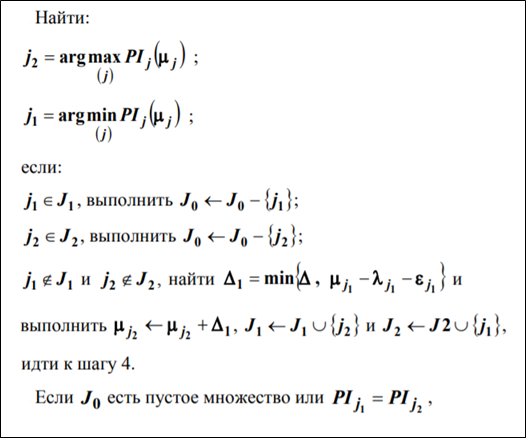
\includegraphics[width=.8\textwidth]{img/alg}
\end{figure}
Как значение $\Delta$ возьмем 0.5.\\По приведенному выше алгоритму определяем множества $J_0, J_1, J_2$. Результаты приведены в таблице \ref{tbl_1}.


\tabulinesep = 1mm
\begin{longtabu} to \textwidth {|X[ c , m ] |X[c , m ] | X[ c , m ]|X[ c , m ]|X[ c , m ]|}\firsthline\hline
№&$J_0$&$J_1$&$J_2$&Действия\\ \hline 
1&1,2,3,4&-&-&$\begin{array}{c} J_1 \leftarrow 1 \\ J_2 \leftarrow 2 \end{array}$ \\ \hline
2&1,2,3,4&1&2&$\begin{array}{c} J_1 \leftarrow 1 \\ J_2 \leftarrow 2 \end{array}$ \\ \hline
3&1,2,3,4&1&2&$\begin{array}{c} J_1 \leftarrow 3 \\ J_2 \leftarrow 2 \end{array}$ \\ \hline
4&1,2,3,4&1,3&2&$\begin{array}{c} J_1 \leftarrow 1 \\ J_2 \leftarrow 2 \end{array}$ \\ \hline
5&1,2,3,4&1,3&2&$\begin{array}{c} J_1 \leftarrow 3 \\ J_2 \leftarrow 4 \end{array}$ \\ \hline
6&1,2,3,4&1,3&2,4&$\begin{array}{c} J_1 \leftarrow 1 \\ J_2 \leftarrow 2 \end{array}$ \\ \hline
7&1,2,3,4&1,3&2,4&$\begin{array}{c} J_0 \leftarrow J_0-1\\ J_0 \leftarrow J_0-2\\ J_1 \leftarrow 2\\ J_2 \leftarrow 1 \end{array}$\\ \hline
8&3,4&1,2,3&1,2,4&$\begin{array}{c} J_1 \leftarrow 4 \\ J_2 \leftarrow 3 \end{array}$ \\ \hline
9&3,4&1,2,3,4&1,2,3,4&$\begin{array}{c} J_0 \leftarrow J_0-3\\ J_0 \leftarrow J_0-4\\ J_1 \leftarrow 3\\ J_2 \leftarrow 4 \end{array}$\\ \hline
10&-&1,2,3,4&1,2,3,4&- \\ \hline
\caption{Формирование множеств J}
\label{tbl_1}
\end{longtabu}
Результаты перераспределения мощностей представлено в таблице \ref{tbl_2}.

\tabulinesep = 1mm
\begin{longtabu} to \textwidth {|X[ c , m ] |X[c , m ] | X[ c , m ]|X[ c , m ]|X[ c , m ]| X[ c , m ]|}\firsthline\hline
№&$\mu_1$&$\mu_2$&$\mu_3$&$\mu_4$&Действия\\ \hline 
1&10&10&10&10&$\begin{array}{c} \mu_2-\Delta \\ \mu_1+\Delta  \end{array}$ \\ \hline
2&10.5&9.5&10&10&$\begin{array}{c} \mu_2-\Delta \\ \mu_1+\Delta  \end{array}$ \\ \hline
3&11&9&10&10&$\begin{array}{c} \mu_2-\Delta \\ \mu_3+\Delta  \end{array}$ \\ \hline
4&11&8.5&10.5&10&$\begin{array}{c} \mu_2-\Delta \\ \mu_1+\Delta  \end{array}$ \\ \hline
5&11.5&8&10.5&10&$\begin{array}{c} \mu_4-\Delta \\ \mu_3+\Delta  \end{array}$ \\ \hline
6&11.5&8&11&9.5&$\begin{array}{c} \mu_2-\Delta \\ \mu_1+\Delta  \end{array}$ \\ \hline
7&12&7.5&11&9.5&$\begin{array}{c} \mu_1-\Delta \\ \mu_2+\Delta  \end{array}$ \\ \hline
8&11.5&8&11&9.5&$\begin{array}{c} \mu_3-\Delta \\ \mu_4+\Delta  \end{array}$ \\ \hline
9&11.5&8&10.5&10&$\begin{array}{c} \mu_4-\Delta \\ \mu_3+\Delta  \end{array}$ \\ \hline
10&11.5&8&11&9.5&- \\ \hline
\caption{Перераспределение мощностей}
\label{tbl_2}
\end{longtabu}

Пересчитаем значения $PI_j, L_j$. Результаты вычисления $PI_j$ приведены в таблице \ref{tbl_3} и \ref{tbl_4}.

\tabulinesep = 1mm
\begin{longtabu} to \textwidth {|X[ c , m ] |X[c , m ] | X[ c , m ]|X[ c , m ]|X[ c , m ]|}\firsthline\hline
№&$PI_1$&$PI_2$&$PI_3$&$PI_4$\\ \hline 
1&	11.5768&0.3252&	3.1492&	0.9483\\ \hline 
2&	4.7354&	0.4186&	3.1492&	0.9483\\ \hline 
3&	2.5586&	0.5589&	3.1492&	0.9483\\ \hline 
4&	2.5586&	0.7835&	1.8443&	0.9483\\ \hline 
5&	1.5990&	1.1769&	1.8443&	0.9483\\ \hline 
6&	1.5990&	1.1769&	1.2098&	1.4138\\ \hline 
7&	1.0931&	1.9623&	1.2098&	1.4138\\ \hline 
8&	1.5990&	1.1769&	1.2098&	1.4138\\ \hline 
9&	1.5990&	1.1769&	1.8443&	0.9483\\ \hline 
10&	1.5990&	1.1769&	1.2098&	1.4138\\ \hline 

\caption{Пересчитанное $PI_j$}
\label{tbl_3}
\end{longtabu}


\tabulinesep = 1mm
\begin{longtabu} to \textwidth {|X[ c , m ] |X[c , m ] | X[ c , m ]|X[ c , m ]|X[ c , m ]| X[ c , m ]|}\firsthline\hline
№&	$L_1$&	$L_2$&	$L_3$&	$L_4$&	L\\ \hline 
1&	4.6255&	0.3665&	2.1179&	0.8937&	8.0038\\ \hline 
2&	2.8172&	0.4381&	2.1179&	0.8937&	6.2669\\ \hline 
3&	1.9765&	0.5347&	2.1179&	0.8937&	5.5229\\ \hline 
4&	1.9765&	0.6709&	1.5434&	0.8937&	5.0845\\ \hline 
5&	1.4944&	0.8743&	1.5434&	0.8937&	4.8059\\ \hline 
6&	1.4944&	0.8743&	1.1930&	1.1491&	4.7109\\ \hline 
7&	1.1840&	1.2051&	1.1930&	1.1491&	4.7313\\ \hline 
8&	1.4944&	0.8743&	1.1930&	1.1491&	4.7109\\ \hline 
9&	1.4944&	0.8743&	1.5434&	0.8937&	4.8059\\ \hline 
10&	1.4944&	0.8743&	1.1930&	1.1491&	4.7109\\ \hline 
\caption{Пересчитанное $L_j$ и $L$}
\label{tbl_4}
\end{longtabu}

\section{Вывод}
В данной работе была произведена оптимизация ССМО, в частности перераспределение мощностей в системе, для уменьшения очереди.\\\\
Начальные значения:\\
$\mu = (10, 10,10, 10)$\\
$L = 8.0038$\\
$L_j= (4.6255, 0.3655, 2.1179, 0.8937)$\\\\
После оптимизации:\\
$\mu = (10.5, 8, 11, 9.5)$\\
$L = 4.7109$\\
$L_j= (1.4944, 0.8743, 1.1930, 1.1491)$\\\\
Как и ожидалась, после оптимизации сети, загруженность системы понизилась.



%------------------------------------------------------------------------------

%\addcontentsline{toc}{section}{Список литературы}
%\bibliography{thesis}
%\bibliographystyle{ugost2008}

\end{document}